%%%%%%%%%%%%%%%%%%%%
% Introduction chapter

%%%%%%%%%%%%%%%%%%%%%%%%%%%%%%%%%%%%%%%%
%%%%%%%%%%%%%%%%%%%%%%%%%%%%%%%%%%%%%%%%
\section{Meiotic recombination overview}
%%%%%%%%%%%%%%%%%%%%%%%%%%%%%%%%%%%%%%%%
%%%%%%%%%%%%%%%%%%%%%%%%%%%%%%%%%%%%%%%%

Meiosis occurs in all sexually reproducing organisms, and is essential to the generation of gametes.
Recombination plays a key role in this process, facilitating the pairing and alignment of chromosomes, while the exchange of genetic material has important implications in inheritance, natural selection, and evolution.

%%%%%%%%%%%%%%%%%%%%%%%%%%%%%%%%%%%%%%%%
\subsection{The biology of meiotic recombination}
%%%%%%%%%%%%%%%%%%%%%%%%%%%%%%%%%%%%%%%%

Prior to meiosis, a diploid cell contains pairs of homologous chromosomes, one of the pair inherited from the father, the other from the mother.
This diploid DNA is replicated just prior to the cell entering the meiotic cycle, in premeiotic S-phase\cite{Bell2002} to generate exact copies of each pair of chromosomes, referred to as sister chromatids.
Meiosis consists of two stages; recombination occurs in the first, meiosis I, while meiosis II sees sister chromatids separate into their respective daughter cells.
Meiosis I is the most complex and lengthy stage, with chromosome pairing, synapsis, and recombination all occurring in succession within prophase I, which is  divided into several sub-stages.

In leptotene (derived from Greek meaning ``thin threads''), changes in chromatin cause the newly replicated chromosomes to form thin individual strands.
Here, the synaptonemal complex (SC), a protein structure that will bind the sister chromatids and their homologues into a tetrad begins to assemble.
The SC consists of a scaffold of proteins that first forms with axial elements that associate with the already paired sister chromatids, solidifying their association.

In the zygotene phase (``paired threads''), pairing between the unraveled DNA begins to occur at regions of homology in a process known as synapsis.
Homologous chromosomes connect to to the SC by transverse filaments, drawing them into the SC structure in a progressive zipper-like mechanism, completing synapsis\cite{Yang2009}.
DNA DSBs occur at this stage (*).

By the pachytene stage (``thick threads''), synapsis, and the SC assembly are fully complete, and the pairs of homologous chromosomes bound within the SC are referred to as a tetrad or bivalent.
Recombination occurs here, mediated by the structure of the SC.
A subset of the DSBs are processed as crossovers, at locations called chiasmata.
The remaining DSBs are repaired through a different pathway, as non-crossovers (gene conversions).

In the diplotene stage (``two threads''), the SC is disassembled, allowing the tetrad to relax slightly.
The homologous chromosomes are still held together at chiasmata locations.

In the final substage of prophase I, diakinesis (``moving through''), the chromosomes condense into visible threads, while the cellular machinery begins to prepare for cell division.
The remaining step of meiosis I are metaphase I, and anaphase I.
Chiasmata, holding the chromosomes together as crossover points are cut, allowing the homologous chromosomes to segregate to their respective cellular poles.

Meiosis II is procedurally similar to mitosis, with different results.
Here, the separation of sister chromatids occurs, producing four haploid gametes.




The recombination process is begun by programmed double strand breaks (DSBs) in the DNA, catalyzed by the protein SPO11, which has a similar function to DNA topoisomerases\cite{DeMassy2013}.
There are two isoforms of \textit{Spo11} in humans, and mice, and a recent study in mice suggests that they may have differing functions, with \textit{Spo11$\beta$} being expressed earlier in meiosis, coinciding with most DSBs occurring on the autosomes.
Male mice with only \textit{Spo11$\beta$} had meiotic defects, with the majority of spermatocytes failing to recombine in the pseudoautosomal region (PAR).
Following this, \textit{Spo11$\alpha$} was found to be expressed later in meiosis, and coincided with DSBs located within the sex chromosomes, including the PAR\cite{Kauppi2011,DeMassy2013}.
This evidence indicates that the initiation of DSBs is a complex, multi-stage process, with autosomal DNA process earlier than DNA from the allosome.




\paragraph{Non-disjunction and the role of recombination.}
In humans, an estimated 30\% of fertilized eggs have aneuploid chromosomes\cite{Hassold2001}, and evidence suggests that meiotic errors are responsible in many cases.
Non-disjunction, the abnormal segregation of chromosomes, can occur at either of the two cell divisions in meiosis.
Meiosis II non-disjunction typically results from a failure of the sister chromatids to separate.
Meiosis I non-disjunction is thought to involve recombination, either in a failure to resolve chiasmata, or a lack of chiasmata entirely.

A reduced recombination rate has been observed in human genetic maps generated from meiosis I aneuploidies (15, 16, 18, 21, XXX, XXY)\cite{Hassold2001,Lynn2004}.
This indicates that recombination rate must remain above a certain level to prevent non-disjunction.
This is supported by the finding that many trisomies involve achiasmate chromosomes, in which recombination is absent in that crhomsome(*).

This supports the idea that chiasmata, which serve to tether homolgous chromosomes together after the dissolution of the SC, and through the first, provide a crucial tension that serves to inhibit non-disjunction.



\afterpage{
\begin{figure}[P]
    \begin{center}
    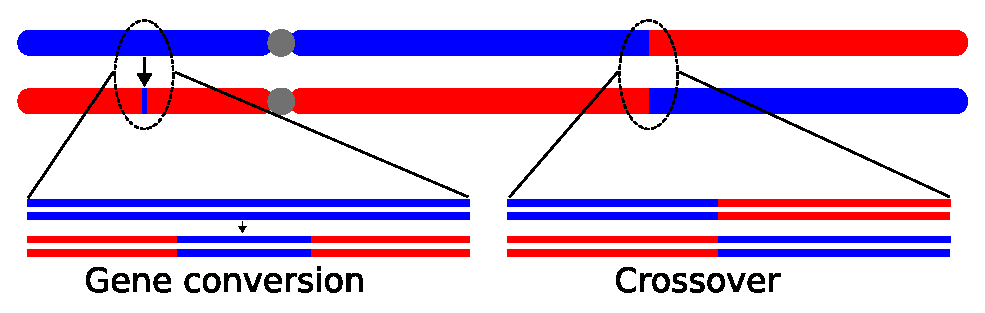
\includegraphics[width=\textwidth]{introduction/figs/outcome_CO-GC}
    \end{center}
    \vspace{-10pt}
    \captionTitle{\textbf{Recombination produces crossover and gene conversion.}}{ 
        Recombination is initiated by DNA double strand breaks that resolve into one of two possible outcomes.
        Crossover (shown at right) is the large-scale, reciprocal exchange of genetic material between two chromosomes around the break point.
        Gene conversion (or non-crossover, shown at left) is the one-way transfer of small amounts of DNA from one chromosome to the other during the repair of the break.
   \label{fig:introOutcomes}}
\end{figure}
\clearpage}



%%%%%%%%%%%%%%%%%%%%%%%%%%%%%%%%%%%%%%%%
\subsection{Timing of meiotic events}
%%%%%%%%%%%%%%%%%%%%%%%%%%%%%%%%%%%%%%%%

%Human:
Oocytes progress through the diplotene stage before undergoing an arrest period.
This arrest is called dictyotene stage, or dictyate.





%%%%%%%%%%%%%%%%%%%%%%%%%%%%%%%%%%%%%%%%
%%%%%%%%%%%%%%%%%%%%%%%%%%%%%%%%%%%%%%%%
\section{Historical overview of meiotic recombination}
%%%%%%%%%%%%%%%%%%%%%%%%%%%%%%%%%%%%%%%%
%%%%%%%%%%%%%%%%%%%%%%%%%%%%%%%%%%%%%%%%

Brief historical review of meiotic recombination, pre Human Genome Project.

%%%%%%%%%%%%%%%%%%%%%%%%%%%%%%%%%%%%%%%%
%%%%%%%%%%%%%%%%%%%%%%%%%%%%%%%%%%%%%%%%
\section{Current status of recombination}
%%%%%%%%%%%%%%%%%%%%%%%%%%%%%%%%%%%%%%%%
%%%%%%%%%%%%%%%%%%%%%%%%%%%%%%%%%%%%%%%%

% Current status of recombination field in humans
%%%%%%%%%%%%%%%%%%%%%%%%%%%%%%
\subsection{Methods for studying recombination}
%%%%%%%%%%%%%%%%%%%%%%%%%%%%%%

Recombination can be observed in a number of ways.
Genome-wide methods have the primary goal of creating a genetic map of the frequency of recombination as a function of physical distance across each chromosome.
In contrast, several other methods are limited in scope, and reveal information about specific loci.
With each method, the detection of recombination is made difficult by the fact that crossovers are rare -- only 20-50 are expected to occur in each meiosis.

% brief introduction to these before describing in detail in "description of approach"
\subsubsection{Pedigree analysis}

Tracing the inheritance of markers from one generation to the next within a family pedigree provided the first genome-wide measurement of recombination across the human genome, prior to the completion of the Human Genome Project.
Early studies used restriction fragment length polymorphism (RFLP) probes to identify specific loci within the genome, and determine if they are linked.
An study described the use of RFLPs to generate a linkage map of recombination in the human genome\cite{Botstein1980}.
Further linkage studies increased the marker density across the genome by using microsatellite, short tandem repeat polymorphisms (STRPs) and other approaches to capturing genetic variation\cite{Morton1991,Matise1994,Dib1996}.
The Marshfield map, generated in 1998 by \citet{Broman1998}, was an important step in characterizing recombination on a genome-wide basis.

With the completion of the Human Genome Project and the publication of the draft sequence of the human genome\cite{Venter2001,Lander2001}, human genetic variation has become increasingly characterized, and a number of technologies have sprung up to make genome-wide ascertainment of variation routine.
Currently, microarray technology provides a well-balanced approach for determining genome-wide coverage of genetic variation.
These arrays target a pre-selected panel of hundreds of thousands to millions of single-nucleotide polymorphisms (SNPs) across every chromosome for a reasonable cost.
While whole-genome sequencing technology allows the discovery of a higher density of markers across the genome, its use is not typically worth the higher cost.
A higher variant coverage will help to narrow the region of uncertainty surrounding a particular crossover, but it will most likely not assist in the detection of additional crossovers in a single meiosis.

Regardless of the method used for obtaining markers, the principle of detecting recombination in a pedigree remains.
Crossovers can be identified by tracing the allele transmissions from parent to child.
Figure \ref{fig:introPedfig} provides a simple visual example, showing a family quartet.
The father in this pedigree has two informative SNPs producing haplotypes 1-1 and 0-0, while the mother is homozygous at both sites.
The male child has a 1-0 haplotype, and therefore must have inherited a recombinant haplotype from his mother.
We can identify here a crossover event and localize that event to an interval flanked by two informative genetic variants.
This region of uncertainty can vary in size and depends on the spacing and genotypes of polymorphic variants within the genome.

\afterpage{
\begin{figure}[p]
    \begin{center}
    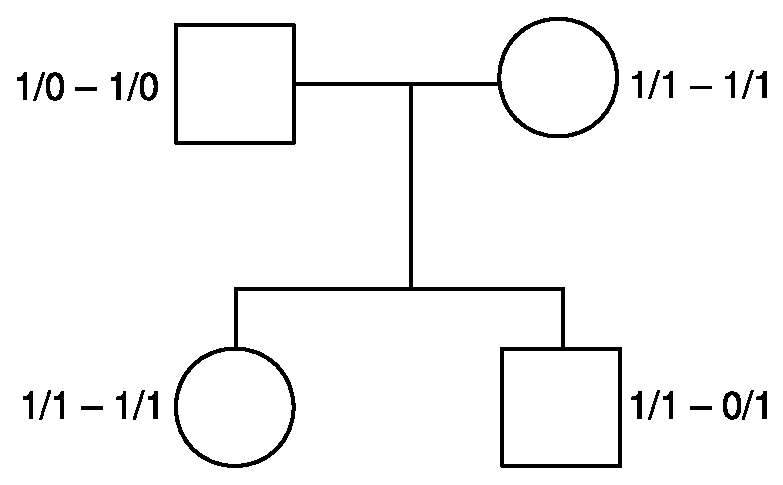
\includegraphics[width=0.75\textwidth]{introduction/figs/pedigree-genotype} \vspace{1cm} \\
    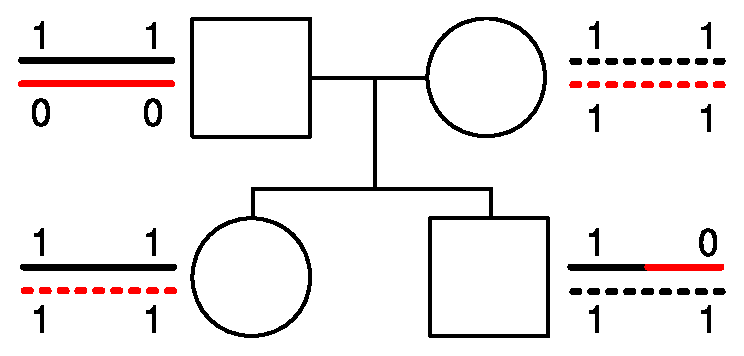
\includegraphics[width=0.8\textwidth]{introduction/figs/pedigree-haplotype}
\end{center}
    \vspace{-10pt}
    \captionTitle{\textbf{Allelic transmission in a family quartet.}}{ 
        The top panel outlines a simple pedigree in which only genotype information is known.
        The bottom panel shows a pedigree for which phase-known haplotype information is known.
        Here, all chromosomes (lines next to each individual) are transmitted in the absence of recombination except for in the male child.  Here there was a recombination event in the father to generate the recombinant chromosome (black/red)
   \label{fig:introPedfig}}
\end{figure}
\clearpage}

% Kong2002,Coop2008,Kong2010

\subsubsection{Linkage disequilibrium approach}

Another powerful method is to use population genetic data to study recombination by inference.
These data can be gathered by genotyping samples of genetic data from unrelated individuals on a microarray or by whole-genome sequencing.

The inference of recombination in such a dataset relies on the quantification of levels of linkage disequilibrium (LD) within the samples, a measurement of linkage between loci.
For example, when alleles at one locus are inherited completely independently of alleles at another locus they are considered to be in linkage equilibrium.
However many alleles exhibit a non-random association, and individuals of the same species tend to share haplotype segments that reflect a shared evolutionary history.
When two alleles on an ancestral haplotype are inherited together they are considered linked, and are not independent of each other.
These alleles exhibit evidence of linkage disequilibrium, a deviation from the assumption of random assortment of alleles.

LD is measured in a pairwise fashion, considering allele frequencies at each pair of markers in the genome.


Hapmap2007, Auton LDhat (Mcvean2004)


\subsubsection{Molecular assays}

A number of molecular assays have been developed for studying recombination.
Most, however are limited to small regions of the genome, and are more effective in males.

\paragraph{Sperm cell assays.}

Sperm typing is one method of identifying both gene conversion and crossover events.

Sperm typing was first used in 1989 to study crossing over in humans\cite{Cui1989}, and uses
allele-specific polymerase chain reaction (PCR) to identify recombination events at a given locus.
In this method, DNA is extracted from multiple haploid sperm cells from a single donor and subject to PCR.
A common reverse primer is used in conjunction with two different allele-specific forward primers, which correspond to polymorphic site in the diploid genome, and are designed to produce different amplicon sizes depending on the matching nucleotide.
Analysis of the PCR products from many sperm cells can reveal the phase of the donor individual, and the recombinant status of each sperm cell.
% \cite{Jeffreys1998,Jeffreys2000,Jeffreys2004}. % first, second(TAP2), review

Sperm typing has been used to produce high-quality data from a number of loci throughout the genome.
One of the first major findings to come out of sperm typing was the characterization of a recombination hotspot in the human major histocompatability complex (MHC), first within one gene, \textit{TAP2}\cite{Jeffreys2000}, then expanded to cover a wider 216 kb region of the MHC\cite{Jeffreys2001}.
All six hotspots found within the region of the MHC were found to be tightly correlated to regions in which LD broke down, providing molecular evidence that recombination hotpots have severe effects on LD patterns.


Jeffreys2009: rise/fall

\citet{Lu2012b}
\citet{Wang2012}


\paragraph{Single oocytes.}
\citet{Hou2013} (single oocytes)


\subsubsection{Recombination initiation maps}
DSB chip: Pratto2014

\subsection{Current ``gold standard'' maps (Hapmap2 LD map, deCODE pedigree map).}

\subsubsection{Marshfield map}
The Marshfield map, generated by \citet{Broman1998} in 1998, was the first genetic map of the human genome at a resolution high enough to make inferences on the recombination properties in humans.
\subsubsection{deCODE maps}
\subsubsection{deCODE maps}

%%%%%%%%%%%%%%%%%%%%%%%%%%%%%%
%%%%%%%%%%%%%%%%%%%%%%%%%%%%%%
\subsection{Sexual dimorphism in recombination.}
%%%%%%%%%%%%%%%%%%%%%%%%%%%%%%
%%%%%%%%%%%%%%%%%%%%%%%%%%%%%%
\paragraph{Heterochiasmy.}

The Marshfield map\cite{Broman1998}, provided some of the first evidence of recombination rate variation across the genome, and between males ane females.
Particularly interesting was the finding that recombination rates are higher in the telomeres, especially in males, and that females have a 1.6-fold higher rate of recombination in the autosomes.

\paragraph{Distribution.}
\paragraph{Differences in SC lenth.}

\subsection{Genes involved in recombination (RFN212, etc)}

PRDM9 (Baudat2010, Berg2011, Hinch2012)

Reynolds2013: mouse RNF212 acts to stabilize meiosis-specific recombination factors including MutS (binds DNA strands and facilitates crossing over).
Rnf212 KO mice are sterile but achieve complete synapsis.

Kong2014: 

RNF212: indentified in Saccharomyces cerevisiae and Caenorhabditis elegans
Kong2008 in humans.

Stefansson2005: Inversion at 17q21.31 increases crossover rate in European females

\subsection{Determinants of recombination placement (PRDM9, GC, chromosome position).}

Differences in populations (Berg2010,Berg2011,Hinch2011)

\subsection{Heritability of recombination rates}
Fledel-Alon2011: male/female rec rates, hotspot usage are heritable.

Ottolini2015: selection for maternal recombination rates. (Kong2004 suggested this as well).

%%%%%%%%%%%%%%%%%%%%%%%%%%%%%%
\subsection{Maternal age effect.}
%%%%%%%%%%%%%%%%%%%%%%%%%%%%%%

Kong2004 (0.082 events/year +/- 0.012 s.e., 4\% increase over 25 years)

Coop2008 (3.1 extra events in mothers over 35 vs mothers under 25.)(0.19 events/year +/- 0.092)

Hussin2011, -0.49 and -0.42 crossovers per year

Bleazard 2013: Decrease in CO \# (n=338 meioses, Asian population)

Martin2015

Polani1991, Rowsey2014: Production line hyp.

\subsection{Recombination in other organisms, including dogs.}

Mouse maps:
Cox2009
Liu2014 (collab cross maps)

\subsection{Heritance of recombination modifiers (rate, etc. Kong)}
\subsection{Sexual dimorphism in recombination rate}

Haldane-Huxley rule: when recombination is absent in one sex, it is the heterogametic sex.

Trivers hypothesis: recombination is lower in the sex that undergoes stronger selection (recombination disrupts favorable haplotypes in the most fit individuals, therefore is selected against).

%%%%%%%%%%%%%%%%%%%%%%%%%%%%%%%%%%%%%%%%
\subsection{Hotspots}
%%%%%%%%%%%%%%%%%%%%%%%%%%%%%%%%%%%%%%%%

\subsubsection{Initial discovery}

Sperm typing produced the first set of well-characterized hotspots in humans, initially focusing within the MHC\cite{Jeffreys2000,Jeffreys2001}.
The correlation of hotspot locations identified by sperm typing in this regions with breakdown of LD measurements provided support for the use of LD methods to find hotspots of recombination genome-wide, without the expense and limitations of single-cell assays\cite{Jeffreys2001}.
In 2005, \citet{Myers2005} produced a fine-scale recombination map in the human genome using LD methods.
Along with this map, hotspots were found to be a ubiquitous feature of the human genome, with a set of $\sim$25,000 found, occurring roughly every 50 kb.
Hapmap LD study expand characterized hotspots throughout the human genome.
These LD studies of recombination also estimated the proportion of recombination occurring within various fractions of the total genome sequence, finding that recombination was intensely concentrated, with 80\% of all recombination occupying less than 20\% of sequence.

Extensive analysis by sperm typing has indicated that hotspots are generally 1-2 kb in width\cite{Jeffreys2004a,Arnheim2003}.


\subsubsection{Discovery of PRDM9}

Since hotspots were first looked at in detail, and the discovery that they were common and spread across the entire genome, questions regarding a possibly regulatory mechanism for hotspots have persisted.
\citet{Myers2005} found that hotspots shared many common features including repeat elements THE1A/B, and a common sequence motif (CCTCCCT) located at the centers of many hotspots.
A further famly of motifs were identified via the use of the Hapmap phase 2 LD map\cite{Hapmap2007}, encompassed by the degenerate 13 bp motif (CCNCCNTNNCCNC)\cite{Myers2008}, estimated to be involved in up to 40\% of all hotspots.

Spencer2006 : hotspots associated with increased GC content, and GC increasing mutations, a likely result of the action of biased gene conversion.


In 2010, a series of papers by three separate groups converged on the identification of PRDM9 from different approaches.
This protein, originally called \textit{Meisetz} was discovered in mice, and is active in early meiotic prophase\cite{Hayashi2005}.
PRDM9 contains a high polymorphic zinc finger DNA binding array, as well as a methyltransferase domain, responsible for the trimethylation of lysine 4 on histone 3 (H3K4).

\citet{Myers2010} compared the sequence of the 13 bp motif against predicted binding of various zinc finger arrays in the genome, finding PRDM9 as a top candidate.
%predicted binding sequence of the PRDM9 zinc-finger array in humans, they found that PRDM9 is a match for the 13 bp sequence motif found at the center of human hotspots.
%Looked at the recombination rate in chimpanzees in sequence surrounding human hotspotso
Using a mouse genetic approach, \citet{Baudat2010} focused on a locus previously determined to be involved in localization of crossover initiation\cite{Grey2009,Parvanov2009},
and narrowed this genomic interval to a region containing the \textit{Prdm9} gene.
A third study used fine mapping techniques in mice to narrow the region, again identifying PRDM9 as the likely candidate protein\cite{Parvanov2010}.



\subsubsection{Hotspots in other species}

Hotspots have been discovered in a number of other species.

Mice contain approximately 15,000-20,000 hotspots, also under the regulation of PRDM9
Mice: Brick2012 (Hotspots via ChIP); Smagulova2011. 15-20,000 total

PRDM9 absent / present

Dogs (Axelsson, Auton2013)

Yeast

Birds


\subsubsection{Conservation between species}
Humans and chimpanzees have a complete absence of hotspot sharing, despite a high degree of overall DNA sequence identity\cite{Ptak2005,Winckler2005,Auton2012a}.

Discuss hotspot paradox vs stable hotspots theory (latter saying hotspots are confined to specific chromosome features (promoters/GC content), as in yeast and dogs)
\subsubsection{Species lacking PRDM9}
Dogs, birds (Singhal2015, biorxiv) 

\subsection{Recombination and disease}

Hussin 2013: Rare allelic forms of PRDM9 associated with childhood leukemogenesis

Turner, D.J. et al. Germline rates of de novo meiotic deletions and duplications causing several genomic disorders. Nat. Genet. 40, 90–95 (2008). \\
Jeffreys, A.J. et al. Complex gene conversion events in germline mutation at human minisatellites. Nat. Genet. 6, 136–145 (1994).

Berg2010:
``PRDM9 status is a major risk factor for de novo CMT1A and HNPP rearrangements, with non-A alleles being strongly protective in N/N individuals, at least in males. Substantial''

PRDM9 knockouts.

%%%%%%%%%%%%%%%%%%%%%%%%%%%%%%%%%%%%%%%%
%%%%%%%%%%%%%%%%%%%%%%%%%%%%%%%%%%%%%%%%
\section{Crossover interference}
%%%%%%%%%%%%%%%%%%%%%%%%%%%%%%%%%%%%%%%%
%%%%%%%%%%%%%%%%%%%%%%%%%%%%%%%%%%%%%%%%

% Current status of crossover interference field.
\begin{titemize}
    \item gamma and two-pathway model, math review.
    \item other methods of measuring coint
    \item genetic map functions taking into account coint Speed,Zhao
    \item potential method of coint action.
    \item Cover what's known in humans, dogs, other organisms.
\end{titemize}

%%%%%%%%%%%%%%%%%%%%%%%%%%%%%%%%%%%%%%%%
%%%%%%%%%%%%%%%%%%%%%%%%%%%%%%%%%%%%%%%%
\section{Gene conversion}
%%%%%%%%%%%%%%%%%%%%%%%%%%%%%%%%%%%%%%%%
%%%%%%%%%%%%%%%%%%%%%%%%%%%%%%%%%%%%%%%%

\begin{titemize}
    \item Review of Li \& Stephens and other models
    \item HMM
    \item Williams paper
\end{titemize}

%%%%%%%%%%%%%%%%%%%%%%%%%%%%%%%%%%%%%%%%
%%%%%%%%%%%%%%%%%%%%%%%%%%%%%%%%%%%%%%%%
\section{Hypothesis and goals}
%%%%%%%%%%%%%%%%%%%%%%%%%%%%%%%%%%%%%%%%
%%%%%%%%%%%%%%%%%%%%%%%%%%%%%%%%%%%%%%%%

% Hypothesis / goal of this thesis.
\begin{titemize}
    \item To investigate specific properties of recombination and how it differs between sexes, individuals, populations, and species.
        %\item To examine how the absence of PRDM9 has affected the recombination landscape in dogs.
    \item To examine how crossover interference varies between individuals and across species.
    \item To further investigate possibilities to model gene conversion in the human genome.
\end{titemize}

%%%%%%%%%%%%%%%%%%%%%%%%%%%%%%%%%%%%%%%%
%%%%%%%%%%%%%%%%%%%%%%%%%%%%%%%%%%%%%%%%
\section{Description of approach}
%%%%%%%%%%%%%%%%%%%%%%%%%%%%%%%%%%%%%%%%
%%%%%%%%%%%%%%%%%%%%%%%%%%%%%%%%%%%%%%%%

% Description of approach.
\subsection{Methods used here to study recombination}
Here, I outline the methods used to study recombination in humans and dogs.

\subsubsection{Linkage disequilibrium}


\subsubsection{Pedigree analysis}

\paragraph{Lander-Green algorithm.}
\paragraph{SHAPEIT2/duoHMM.}

\subsection{Models of crossover interference}
    Models of crossover interference (described in full in nat comm paper).

\subsection{Gene conversion HMM}
    Gene conversion in admixed populations HMM \& statistical methods for recombination modeling.


%%%%%%%%%%%%%%%%%%%%%%%%%%%%%%%%%%%%%%%%
%%%%%%%%%%%%%%%%%%%%%%%%%%%%%%%%%%%%%%%%
\renewcommand{\bibname}{References}
\bibliographystyle{ccampbell_thesis} %unsrtnat} %abbrvnat_noURL} %abbrvUnsrt_last-first} %plain,unsrt,alpha,abbrv,acm,apalike,unsrt
\begingroup
    \setlength{\bibsep}{10pt}
    \linespread{1}\selectfont
    \bibliography{/home/ccampbell/Dropbox/papers/recombination,/home/ccampbell/Dropbox/papers/thesis}
\endgroup
%%%%%%%%%%%%%%%%%%%%%%%%%%%%%%%%%%%%%%%%
%%%%%%%%%%%%%%%%%%%%%%%%%%%%%%%%%%%%%%%%

